
\section{ESP8266}
\label{sec:ESP8266}

O ESP8266 é um SOC (\emph{System On a Chip} - Sistema em um \emph{Chip}),
ou seja, é um chip com todos os componentes lógicos
eletrônicos necessários e partes para um dado sistema em único cirtuito
integrado. Este chip possui:


\begin{alineas}
	\item \emph{Wi-Fi} embutido com capacidade de 2,4 GHz (802.11 b/g/n);

	\item 16 GPIOs (\emph{general-purpose input/output}) incluindo interfaces
 I2U, SPI, UART, entrada ADC, saída PWM;

	\item Arquitetura \emph{RISC} de 32 bits;

	\item CPU que opera em  80 MHz, com possibilidade de operar em 160 MHz;

	\item 64 KB de ROM para \emph{boot};

	\item 64 KB de RAM para instruções;

	\item 96 KB de RAM para dados;

	\item Memória \emph{Flash SPI} de 512 KB a 4 MB (dependente de módulo externo);

	\item Núcleo baseado no \emph{IP Diamand Standard LX3} da \emph{Tensilica}.

\end{alineas}

Para o mercado de prototipação, fabricantes constroem placas de diferentes configurações com
este chip como elemento central, os chamados módulos. Estes módulos usam o
ESP8266 com diferenças perceptíveis, por exemplo, quantidade de pinos, dimensões
físicas e alguns podem até operar de modo \emph{standalone} (sem outro \emph{hardware} de
suporte como reguladores de tensão, conversores serial-USB) e especialmente a
 \emph{Memória Flash SPI}. Neste trabalho, foram usados os módulos:
\emph{ESP-01}, \emph{LoLin}, \emph{D1 mini} e \emph{ESP-12f} com placa adaptadora de pinos.


\begin{figure}[htb]
	\caption{\label{fig:modelos-esp}Módulos ESP8266}
	\begin{center}
		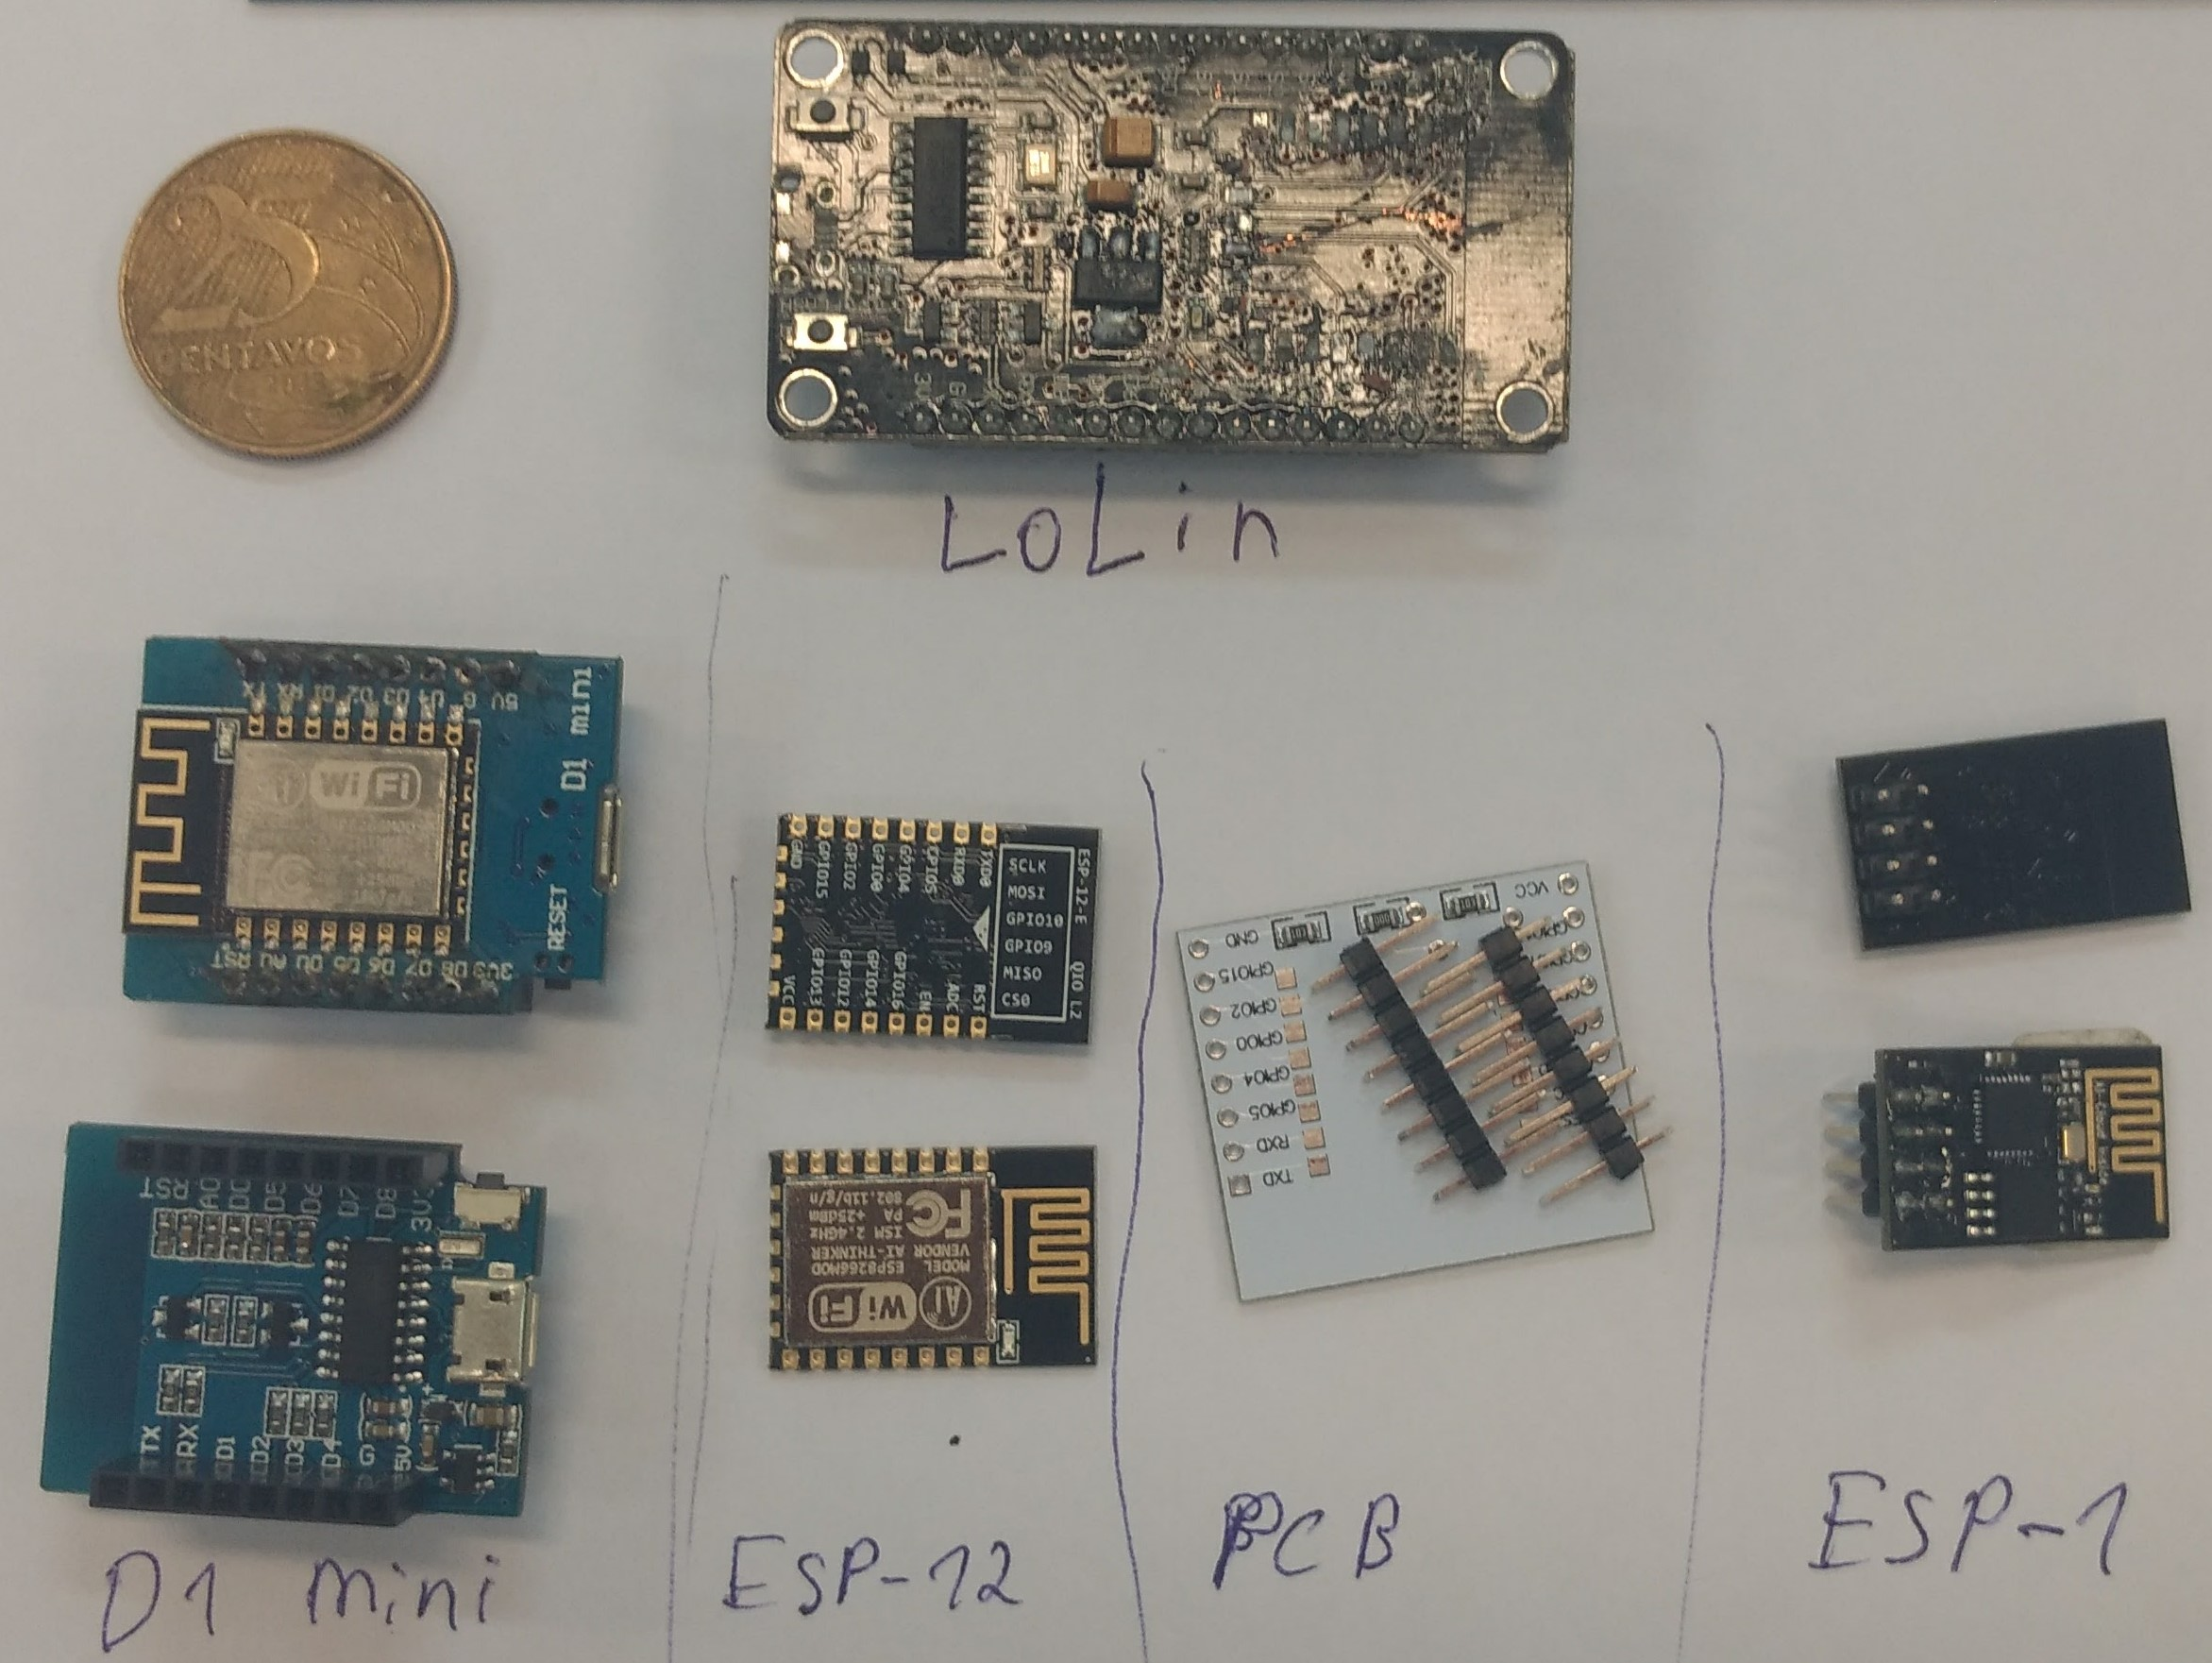
\includegraphics[width=1\textwidth]{040-plataformas/esp-dev/modulos-esp.jpg}
	\end{center}
	\legend{Fonte: Elaborada pelo autor}
\end{figure}



\subsection{Disponibilidade no mercado}
\label{subsec:mercado-esp}

As diferentes especificações implicam em diferentes produtos e mercado para
eles, isto resulta em diferentes custos em diferentes regiões.

\begin{table}[htb]
\IBGEtab{%
\ABNTEXchapterfont {
  \caption{Descrição e custos de módulos ESP8266}%
  \label{table:custo-esp}
}
}{%
\begin{tabular}{cccc}
\toprule
Módulo				&	Pinos de GPIO e conectores							&	Memória	&	Custo			\\
\midrule \midrule
ESP-01				&	8 pinos macho, incompatível com \emph{breadboard}	&			&  \\
					&	(GND, 3v3, TX, RX, CH_PD, RST, GPIO 0, GPIO 2)		&	1 MB	&	R\$ 16,80 		\\
\midrule
ESP-12f				&	22 pontos para montagem em superficie, nenhum pino	&	4 MB	&	R\$ 14,90 		\\
\midrule
D1 mini (ESP-12f)	&	16 + microUSB										&	4 MB	&	R\$ 12,56^{1}	 \\
\midrule
LoLin (ESP-12f)		&	30 + microUSB										&	4 MB	&	R\$ 35,87 		\\
\midrule
\bottomrule
\end{tabular}%
}{%
	\fonte{Produzido pelo autor.}%
	\nota[Nota 1]{D1 mini (ESP-12f) foi adquirido do mercado chinês.}%
}
\end{table}

\begin{table}[htb]
\IBGEtab{%
\ABNTEXchapterfont {
  \caption{Descrição e custos de acessórios para ESP8266}%
  \label{table:acessorios-esp}
}
}{%
\begin{tabular}{ccc}
	\toprule
	Acessórios						&	Descrição									&	Custo			\\
	\midrule
	Esp8266 Placa Para Soldar		& Placa com 16 pinos conectados aos				&					\\
	Esp-07, Esp-08, Esp-12, Esp-12e	& pontos de superficie do ESP-12f				&	R\$ 3,45 		\\
	\midrule
	Conversor Usb Serial 			&	Fornece uma conexão serial-USB entre		& 	 				\\
	Ch340 Rs232 - 3,3v 5v^{1}		&	o ESP8266 e o computador de desenvolvimento	&	R\$ 6,87 		\\
	\midrule
	Adaptador Usb Serial			&	Fornece uma conexão serial-USB entre		&		\\
	Ttl Conversor Cp2102^{2}		&	o ESP8266 e o computador de desenvolvimento	&	R\$ 20,00		\\
	\midrule
	Ams1117 3,3v (3.3v) - Lm1117	&	Regula a tensão de uma USB ou pilhas para	&		\\
									&	3.3\emph{V} 1\emph{A} usado nos módulos		&	R\$ 14,99 (10 unidades) \\
	\midrule
\bottomrule
\end{tabular}%
}{%
	\fonte{Produzido pelo autor.}%
	\nota[Nota 1]{Compatível apenas com \emph{Windows 7}.}%
	\nota[Nota 2]{Compatível com \emph{Windows 10} e com o computador de desenvolvimento.}%
}
\end{table}


A escolha do ESP8266 como primeira tentativa devido o seu baixo custo e de
tamanho reduzido. No exterior, ele pode ser encontrado por de USD\$ 1,76 a 2,2
\cite{AlibabaESP}, e no Brasil por aproximadamente BRL R\$ 15,00 \cite{mercadolivreEsp}.

Devido ao seu tamanho, ele é de fácil integração com demais dispositivos,
bastando o uso de uma comunicação serial. Já sobre a comunidade, há inúmeros
projetos DIY (em inglês \emph{do it yourself}, em português "faça você mesmo")
que ensinam a como construir e manipular projetos que envolvem diferentes
módulos. Além disso, a empresa  idealizadora e fabricante do chip, Espressif,
disponibiliza no GitHub projetos com documentação e código aberto.

Para desenvolver na plataforma, os módulos ESP foram utilizados de formas
diferentes dependendo das capacidades de cada módulo. Quando o módulo possuía
regulador de tensão embarcado, utilizava-se o próprio conectado a uma porta USB.
Quando o módulo não possuía tal, utilizava-se um circuito com fonte externa
(pilhas ou USB) e um regulador de tensão conectados aos pinos \emph{3v3} e
\emph{GND}. Depedendo da complexidade do circuito para ligar e ter acesso à
serial do módulo, é necessário o uso de uma placa \emph{breadboard}, como na
\autoref{fig:esp-pilha-serial}. Para este trabalho foi utilizado o regular
\emph{AMS1117 3v3} e dois capacitores de $100 \mu F$.

\begin{figure}[htb]
	\caption{\label{fig:esp-pilha-serial}ESP-12f com regulador tensão e serial}
	\begin{center}
		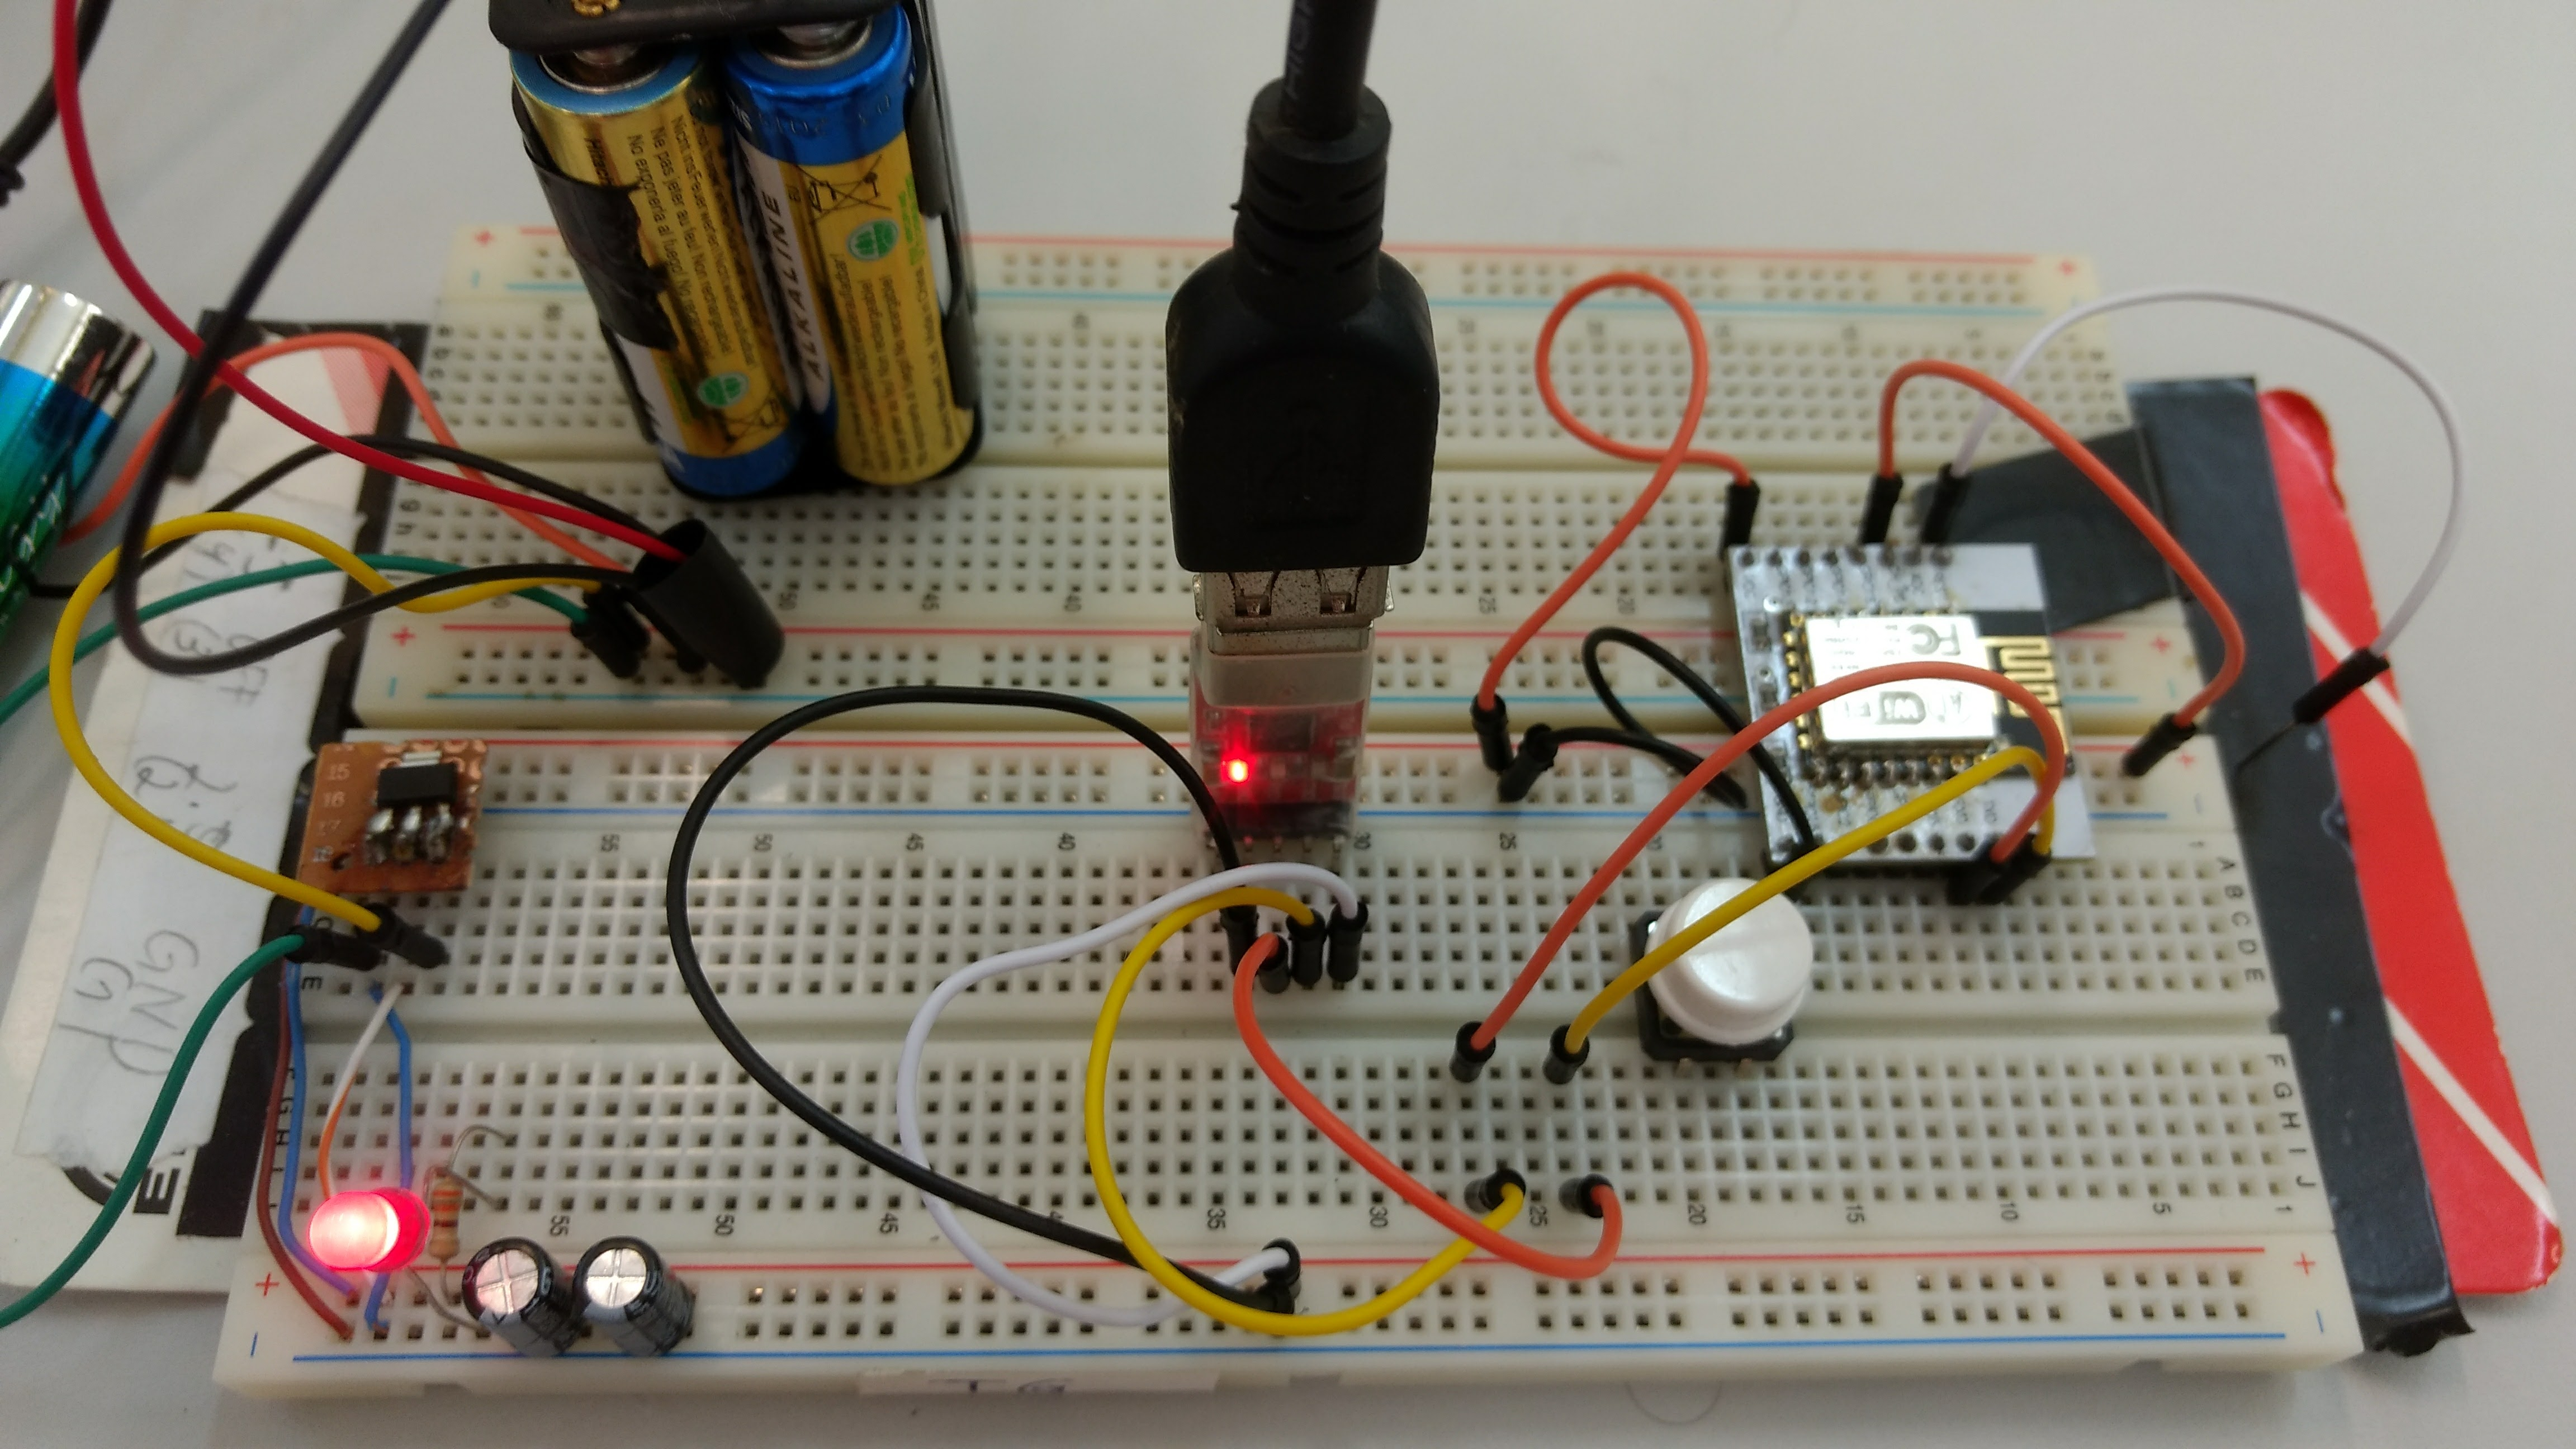
\includegraphics[width=1\textwidth]{040-plataformas/esp-dev/breadboard.jpg}
	\end{center}
	\legend{Fonte: Elaborada pelo autor}
\end{figure}


\subsection{Desenvolvimento e Implantação}
\label{subsec:dev-esp}

Todo código produzido em uma linguagem de programação é compilado por uma
ferramenta e, então, carrega-se os arquivos binários para o ESP8266 através da
serial, para que a execução do código seja iniciada. Na
\autoref{fig:esp-toolchain}, é apresentado um modelo de desenvolvimento e
implantação desde o código até chegar no módulo ESP e, também, a lista de
carregadores usados.

\begin{figure}[htb]
	\caption{\label{fig:esp-toolchain}ESP-12f com regulador tensão e serial}
	\begin{center}
		\begin{verbatim}
		+--------+           +-----------+
		| Código |-----------> Compilador|
		+--------+           |           |      +----------------------+
		                     |  Ligador  <------| Cabeçalhos Espressif |
		                     +-----------+      +----------------------+
		                           |
		+------------+        +----v-----+
		| Carregador <--------+ Binários |
		+-----+------+        +----------+
		       \
		        \---Serial
		         \
		+---------v----+
		|  Módulo ESP  |
		+--------------+
		\end{verbatim}
	\end{center}
	\legend{Fonte: Elaborada pelo autor}
\end{figure}


\begin{table}[htb]
\IBGEtab{%
\ABNTEXchapterfont {
	\caption{Ferramentas para desenvolvimento com ESP8266}%
	\label{table:tools-esp}
}
}{%
\begin{tabular}{cccc}
	\toprule
	Ferramenta			&	Editor	&	Compilador e Ligador	&	Carregador	\\
	\midrule \midrule
	Arduino IDE			&	Sim		&	arduino C				&	Sim, mas não carrega binários pré compilados	\\
	\midrule
						&			&	NodeMCU Lua,			&		\\
	ESPlorer			&	Sim		&	MicroPython,			&	Não, conta com firmware específico	\\
						&			&	AT e RN2483				&		\\
	\midrule
	esptool.py			&	Não		&	Não 					&	Somente binários pré compilados	\\
	\midrule
	ESP8266 Flash		&			&							&		\\
	Downloader			&	Não		&	Não 					&	Somente binários pré compilados	\\
	\midrule
	NodeMCU Firmware	&			&							&		\\
	Programmer			&	Não		&	Não 					&	Somente binários pré compilados	\\
	\midrule
	\bottomrule
\end{tabular}%
}{%
	\fonte{Produzido pelo autor.}%
}
\end{table}

Todo código produzido é carregado para o módulo ESP através de seu barramento
serial. Alguns modelos, como o \emph{LoLin} e \emph{D1 mini}, já apresentam
conversor serial para \emph{micro-USB}. Para os que não possuem tal interface é
necessário utilizar um conversor serial-USB externo, a
\selfef{fig:esp-pilha-serial} demonstra esse método.

As \emph{GPIOs} do \emph{ESP-12f} são acessadas somente através de placas
de circuito impresso, então uma foi adquirida para a programação do mesmo.

Dos conversores serial-USB adquiridos, o modelo \emph{CH340G} não funcionou por
não ter driver compatível com o \emph{Windows 10}, em contraste com o modelo
\emph{CP2102}  que funcionou no mesmo sistema operacional.


\subsection{Testes e resultados}
\label{subsec:mercado-esp}

O primeiro objetivo durante a programação dos módulos ESP8266 é cumprir a
premissa  estabelecida no início deste capítulo de acessar o Modo Promíscuo da
interface Wi-Fi. Neste caso, procurou-se pelo ponto da \emph{API} de
\emph{hardware} do ESP8266 onde os pacotes destinados a outros dispositivos são
descartados, desativar este filtro, capturar e avaliar o pacote para localizar o
seu emissor.

A principio, com o \emph{firmware AT} que é o padrão do módulo ESP-01 e com o
emulador de serial da \emph{Arduino IDE} ou a aplicação \emph{Cool Term} é
possível configurar e utilizar o módulo por completo apenas com instuções AT
enviadas através da conexão serial. A primeira investigação sobre a API do protocolo
AT indicou \citeonline{room15} como uma fonte sucinta da documentação
oficial fornecida por \citeonline{espressifATwiki} do \emph{firmware AT} e
não revelou nenhuma capacidade de ativar o Modo Promíscuo.

Também utilizou-se a linguagem C que foi compilada na \emph{Arduino IDE} e
enviada ao ESP8266 com a extenção \emph{esp8266 by ESP8266 Community} que inclui
os cabeçalhos de funções para que o compilador padrão da \emph{Arduino IDE} gere
código  executável pelo ESP8266. Mesmo nesta API, nenhuma capacidade de ativar o
Modo Promíscuo foi encontrada.

\begin{figure}[htb]
	\caption{\label{fig:esp-arduino}Código em C compilado e implantado em um ESP8266}
	\begin{center}
		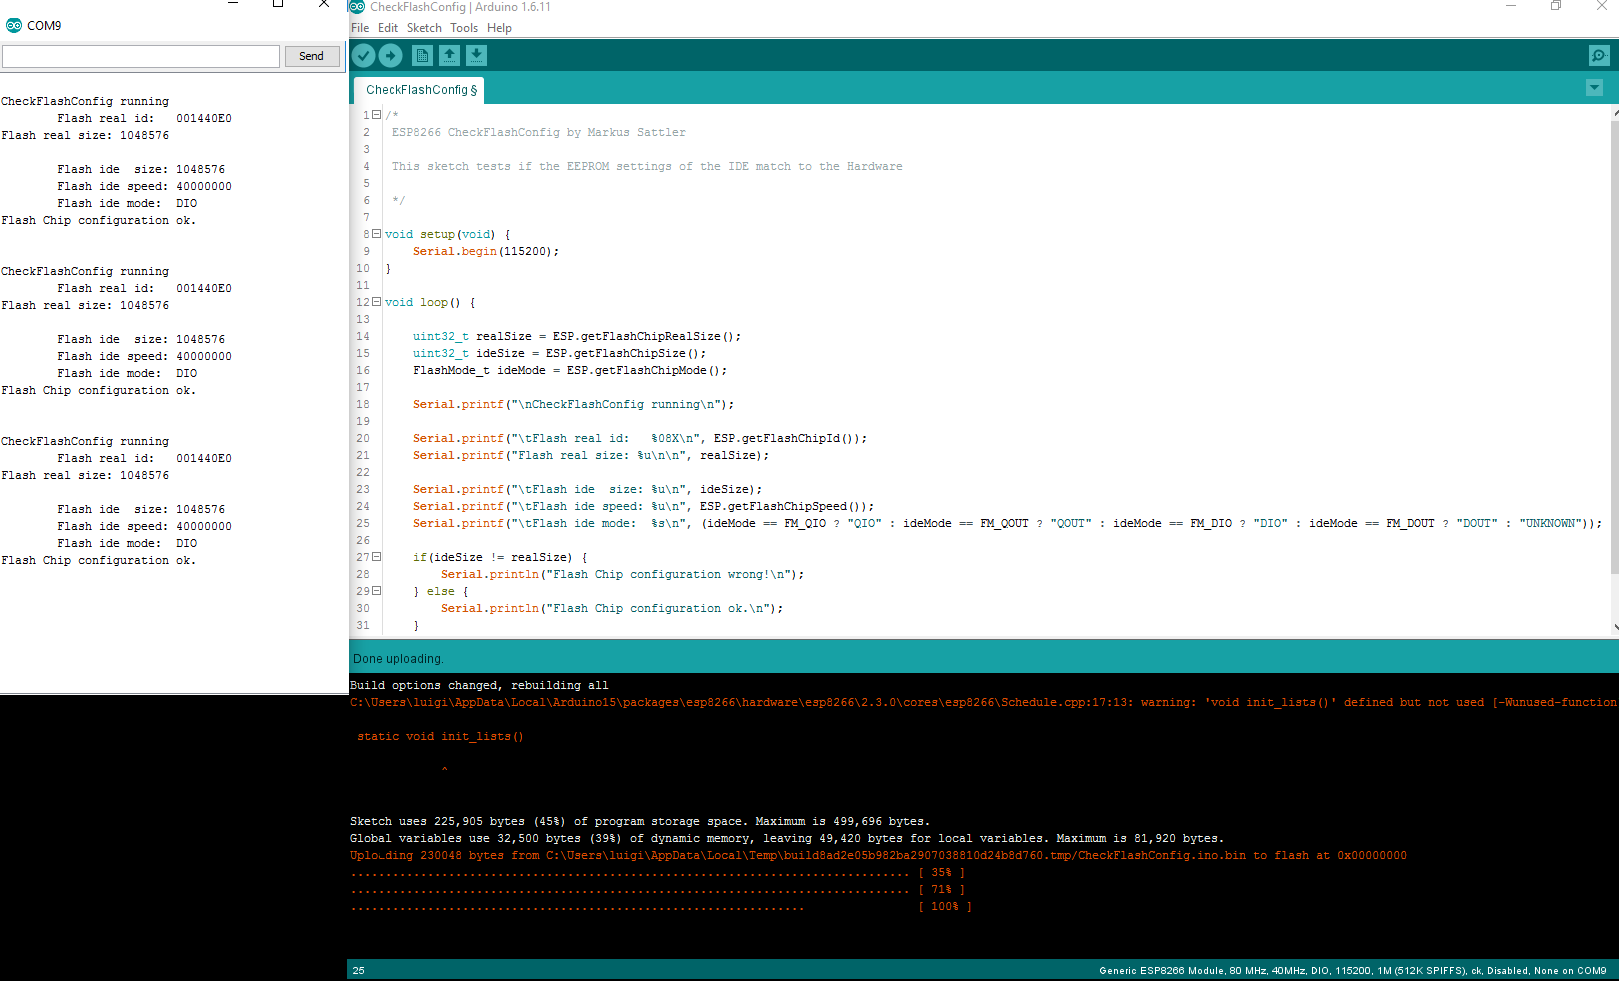
\includegraphics[width=1\textwidth]{040-plataformas/esp-dev/arduino-ide.png}
	\end{center}
	\nota[Esquerda]{Comandos AT no emulador de serial da \emph{Arduino IDE}.}%
	\nota[Direita]{Editor da \emph{Arduino IDE} com código C.}%
	\nota[Abaixo em preto]{Processo de \emph{upload} do firmware escrito em C.}%
	\fonte{Elaborado pelo autor.}%
\end{figure}


Nova tentativa para a programação  dos módulos escolhidos foi feita através de
\emph{toolchains} (conjunto de ferramentas para desenvolvimento de software) da
empresa \emph{Espressif} e de um usuário do \emph{Github}, muito utilizado para
projetos de ESPs, \citeonline{Pfalcon}. Ambas as \emph{toolchains}
são \emph{SDKs} de código aberto. Os \emph{scripts} foram feitos na linguagem C,
compilados nessas SDKs e transferidos para os módulos ESP. Neste caso,
a configuração delas mostrou-se um desafio pois requisitavam uma versão
específica do \emph{Ubuntu Linux} que a máquina utilizada para o desenvolvimento
não suporta. Também foi testada a utilização de máquinas virtuais mas, novamente,
a máquina do desenvolvedor não possui virtualização impossibilitando esta opção.

Em conclusão, apesar do baixo custo e documentação da comunidade aberta, o
ESP8266 não foi adotado como sensor, pois não foi possível colocá-lo em modo
prosmícuo, essencial para detectar pacotes entre dispositivo e os pontos de
acesso inviabilizando completamente o uso desta plataforma mesmo esta sendo a
mais adequada e promissora no ponto de vista da construção de um produto final
por seu extremo baixo custo.
